\documentclass[11pt,a4paper]{article}

% ------------------------------------------------------------
% Packages
% ------------------------------------------------------------
\usepackage[margin=1in]{geometry}
\usepackage{amsmath,amssymb,amsfonts}
\usepackage{booktabs}
\usepackage{tabularx}
\usepackage{longtable}
\usepackage{multirow}
\usepackage{array}
\usepackage{graphicx}
\usepackage{float}
\graphicspath{{figures/}}
\usepackage{xcolor}
\usepackage{hyperref}
\usepackage{enumitem}
\usepackage{caption}
\usepackage{subcaption}
\usepackage{listings}
\usepackage{tikz}
\usetikzlibrary{arrows.meta,positioning,shapes.geometric}

\hypersetup{
  colorlinks=true,
  linkcolor=blue!50!black,
  urlcolor=blue!50!black,
  citecolor=blue!50!black
}

\lstset{
  basicstyle=\ttfamily\small,
  breaklines=true,
  frame=single,
  backgroundcolor=\color{gray!8},
  columns=fullflexible
}

\title{%
  Hippocampal Neuropixels Simulation\\
  and Causal Manifold Decoding%
}
\author{Technical project document\\[0.5em]
\large\texttt{hippo} repository}
\date{\today}

\begin{document}
\maketitle

\begin{abstract}
This document specifies a Python research pipeline that (i)~simulates hippocampal single-unit activity during open-field navigation, (ii)~records it through a Neuropixels-like probe with sorting degradation, and (iii)~decodes behavioral latent variables from \emph{causal} population spike counts.
Hyperparameter search over decoder models, integration windows, and optional manifold features is performed automatically; the selected configuration is then replayed in a closed-loop causal setting.
We document the neural rate equations, probe anatomy, causal decoding architecture, decoder model zoo, and manifold feature modes with explicit mathematical definitions and default numerical parameters.
\end{abstract}

\tableofcontents
\newpage

% ============================================================
\section{Introduction and scientific framing}
% ============================================================

The simulator knows the true behavioral state.
The decoder observes only spike times (ground-truth Poisson spikes or spikes after Neuropixels-like degradation and sorting).
Comparing these two spike sources quantifies information loss due to extracellular recording and sorting.
Searching causal integration windows asks how much recent neural history is required to decode spatial, proprioceptive, and contextual variables.
Searching decoder families asks which estimator best extracts those latents from population activity.
Closed-loop replay tests whether decoded estimates can drive realtime triggers.

Six computational operations are kept conceptually separate:
\begin{enumerate}[leftmargin=*]
  \item population partition (which units enter a model);
  \item observation construction (causal spike counts);
  \item manifold geometry (map to latents $z_t$);
  \item temporal dynamics on the manifold (history of length $L$);
  \item behavioral decoding ($\hat y_{t+\tau}$);
  \item interregional communication (planned).
\end{enumerate}

% ============================================================
\section{Public software workflow}
% ============================================================

The intended user interface consists of three scripts:
\begin{enumerate}[leftmargin=*]
  \item \texttt{run\_simulation.py} --- generate behavior, rates, spikes, recording, sorting;
  \item \texttt{run\_full\_decoder\_workflow.py} --- compare models/windows, select the best configuration, run closed-loop replay, optionally plot;
  \item \texttt{run\_visualizations.py} --- regenerate figures from saved outputs only (never retrains).
\end{enumerate}

\begin{lstlisting}[language=bash,caption={Standard end-to-end commands.}]
python run_simulation.py \
    --output outputs/ratinabox_002 \
    --seed 2 \
    --neural-backend ratinabox_neurons

python run_full_decoder_workflow.py \
    --input outputs/ratinabox_002 \
    --output outputs/ratinabox_002 \
    --compare-sources \
    --closed-loop-target spatial_context \
    --selection-policy shortest_near_optimal \
    --compile-pdf

python run_visualizations.py \
    --experiment outputs/ratinabox_002 \
    --all --compile-pdf
\end{lstlisting}

Hyperparameter tuning is intentionaly \emph{internal} to the decoder workflow: users need not manually choose $W$ or call separate comparison/replay scripts for the standard path.

\begin{figure}[h]
\centering
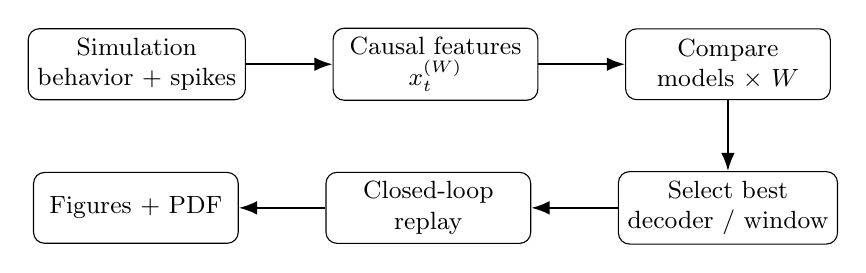
\begin{tikzpicture}[
  node distance=0.9cm and 1.1cm,
  box/.style={draw, rounded corners, align=center, minimum width=2.6cm, minimum height=0.9cm, font=\small},
  arr/.style={-{Latex}, thick}
]
\node[box] (sim) {Simulation\\behavior + spikes};
\node[box, right=of sim] (feat) {Causal features\\$x_t^{(W)}$};
\node[box, right=of feat] (cmp) {Compare\\models $\times$ $W$};
\node[box, below=of cmp] (sel) {Select best\\decoder / window};
\node[box, left=of sel] (rt) {Closed-loop\\replay};
\node[box, left=of rt] (viz) {Figures + PDF};
\draw[arr] (sim) -- (feat);
\draw[arr] (feat) -- (cmp);
\draw[arr] (cmp) -- (sel);
\draw[arr] (sel) -- (rt);
\draw[arr] (rt) -- (viz);
\end{tikzpicture}
\caption{High-level pipeline. Tuning and selection occur under the hood before realtime replay.}
\label{fig:pipeline}
\end{figure}

% ============================================================
\section{Simulation pipeline}
% ============================================================

Default session duration is $600\,\mathrm{s}$ (10 minutes). Behavior and rate updates run at $20\,\mathrm{Hz}$ ($\Delta t = 0.050\,\mathrm{s}$).

\begin{enumerate}[leftmargin=*]
  \item \textbf{Behavior:} RatInABox open-field trajectory (thigmotaxis, stalls, smooth turns).
  \item \textbf{Features:} place, head direction, speed, acceleration, boundary distance, theta phase, ripple.
  \item \textbf{Rates:} custom CA1/CA2/CA3/DG equations \emph{or} RatInABox neuron classes.
  \item \textbf{Spikes:} inhomogeneous Poisson sampling (ground truth).
  \item \textbf{Recording:} multi-channel templates, noise, motion amplitude drift, collisions.
  \item \textbf{Sorting:} Kilosort-like re-extraction with misses, jitter, contamination.
\end{enumerate}

\subsection{Neural backends}
\begin{description}[leftmargin=*]
  \item[\texttt{custom\_rate\_equations}] Explicit hippocampal rate model (Section~\ref{sec:rates}).
  \item[\texttt{ratinabox\_neurons}] RatInABox place / HD / boundary / speed cells mapped onto anatomical units (recommended for quick experiments).
\end{description}

Primary simulation outputs: \texttt{behavior.csv}, \texttt{units.csv}, \texttt{spikes\_ground\_truth.csv}, \texttt{spikes\_sorted.csv}, \texttt{anatomy\_regions.csv}, \texttt{summary.json}.

% ============================================================
\section{Neural rate model}
\label{sec:rates}
% ============================================================

Source of truth in code: \texttt{hippo\_sim/rate\_equations.py}, \texttt{hippo\_sim/config.py}.

\subsection{Dynamics}
For each unit $i$, rates $R_i(t)$ obey the linear filter
\begin{equation}
  \tau_i \frac{dR_i}{dt} = -R_i + \lambda_i^{\mathrm{target}}(t),
  \label{eq:rate-ode}
\end{equation}
integrated with Euler steps at the behavioral timestep $\Delta t = 0.05\,\mathrm{s}$.

\subsection{Target drive}
Let $p(t)$ be allocentric position, $\theta(t)$ head direction, $v(t)$ speed, $a(t)$ acceleration, $d_{\mathrm{wall}}(t)$ distance to the nearest wall, $\phi_\theta(t)$ theta phase, and $r(t)$ a ripple envelope.
Define
\begin{align}
  f_i^{\mathrm{place}}(t)
  &= \exp\!\Bigl(-\frac{\|p(t)-p_{0,i}\|^2}{2\sigma_i^2}\Bigr),
  \label{eq:fplace}\\
  f_i^{\mathrm{HD}}(t)
  &= \frac{\exp\!\bigl(\kappa_i\cos(\theta(t)-\theta_i^{\mathrm{pref}})\bigr)}
         {\exp(\kappa_i)/I_0(\kappa_i)},
  \label{eq:fhd}\\
  f_i^{\mathrm{speed}}(t)
  &= \frac{\max\bigl(0,\, v(t)-v_i^{\mathrm{thresh}}\bigr)}{30-v_i^{\mathrm{thresh}}},
  \label{eq:fspd}\\
  f_i^{\mathrm{acc}}(t)
  &= \mathrm{clip}\!\bigl(|a(t)|/50,\,0,\,1\bigr),
  \label{eq:facc}\\
  f_i^{\mathrm{bnd}}(t)
  &= \exp\!\Bigl(-\frac{d_{\mathrm{wall}}(t)^2}{2\cdot 15^2}\Bigr),
  \label{eq:fbnd}\\
  f_i^{\theta}(t)
  &= 1 + w_i^{\theta}\cos\phi_\theta(t).
  \label{eq:ftheta}
\end{align}
The multiplicative drive is
\begin{align}
  \mathrm{drive}_i(t)
  &=
  b_i
  + A_i\, f_i^{\mathrm{place}}
  \,(1+w_i^{\mathrm{HD}} f_i^{\mathrm{HD}})
  \,(1+w_i^{\mathrm{speed}} f_i^{\mathrm{speed}})
  \,(1+0.2\, f_i^{\mathrm{acc}})
  \, f_i^{\theta}
  \nonumber\\
  &\quad
  + w_i^{\mathrm{bnd}} A_i f_i^{\mathrm{bnd}}
  + w_i^{\mathrm{ripple}} A_i r(t).
  \label{eq:drive}
\end{align}
Region-specific modifications:
\begin{itemize}[leftmargin=*]
  \item \textbf{CA3:} $\mathrm{drive}_i \leftarrow \mathrm{drive}_i + w_i^{\mathrm{rec}}\,\overline{R}(t)$.
  \item \textbf{DG sparsity:} if
  $f_i^{\mathrm{place}}(1+w_i^{\mathrm{speed}} f_i^{\mathrm{speed}}) < \theta_i^{\mathrm{sparse}}$,
  then $\mathrm{drive}_i \leftarrow 0.1\, b_i$.
\end{itemize}
Finally
\begin{equation}
  \lambda_i^{\mathrm{target}}(t)
  =
  \max\bigl(\mathrm{drive}_i(t)\,\xi(t)\,g_i(t),\, 0\bigr),
\end{equation}
where $\xi(t)$ is a shared arousal/state Ornstein--Uhlenbeck (OU) factor and $g_i(t)$ is a per-unit gain OU process.

\subsection{Default parameters}
\begin{table}[h]
\centering
\caption{Rate parameters by cell type.}
\label{tab:rate-params}
\small
\begin{tabular}{@{}lrrrrl@{}}
\toprule
Parameter & CA1\_pyr & CA2\_pyr & CA3\_pyr & DG\_granule & Units \\
\midrule
$\tau$ & 0.05 & 0.05 & 0.06 & 0.08 & s \\
$b$ (baseline) & 0.5 & 0.4 & 0.3 & 0.05 & Hz \\
$A$ (amplitude) & 12.0 & 10.0 & 8.0 & 15.0 & Hz \\
$\sigma_{\mathrm{place}}$ & 10 & 8 & 12 & 6 & cm \\
$w_{\mathrm{HD}}$ & 0.4 & 0.35 & 0.2 & 0.1 & --- \\
$\kappa_{\mathrm{HD}}$ & 2.0 & 2.5 & 1.5 & 1.0 & --- \\
$w_{\mathrm{speed}}$ & 0.3 & 0.25 & 0.2 & 0.5 & --- \\
$v_{\mathrm{thresh}}$ & 2 & 2 & 2 & 3 & cm/s \\
$w_\theta$ & 0.25 & 0.15 & 0.1 & 0.05 & --- \\
$w_{\mathrm{ripple}}$ & 0.5 & 0.1 & 0.6 & 0.0 & --- \\
$w_{\mathrm{boundary}}$ & 0.2 & 0.15 & 0.1 & 0.3 & --- \\
$w_{\mathrm{recurrent}}$ & --- & --- & 0.15 & --- & --- \\
$\theta_{\mathrm{sparse}}$ & --- & --- & --- & 0.3 & --- \\
\bottomrule
\end{tabular}
\end{table}

\begin{table}[h]
\centering
\caption{Drift, recording, and sorting defaults.}
\label{tab:drift-rec}
\small
\begin{tabular}{@{}lll@{}}
\toprule
Parameter & Value & Units / notes \\
\midrule
Place drift SD & 0.1 & cm/min \\
Place update interval & 30 & s \\
State OU $\tau$, $\sigma$ & 120, 0.15 & s, --- \\
Gain OU $\tau$, $\sigma$ & 180, 0.1 & s, --- \\
Channels / pitch & 384 / 20 & --- / $\mu$m \\
Sample rate & 30 & kHz \\
Template span & 3--10 & channels \\
Amplitude range & 20--200 & $\mu$V \\
Noise SD & 15 & $\mu$V \\
Miss rate / jitter & 0.12 / 0.3 & --- / ms \\
Contamination / merge & 0.08 / 0.04 & --- \\
\bottomrule
\end{tabular}
\end{table}

% ============================================================
\section{Probe anatomy}
% ============================================================

Neuropixels 1.0 single-shank geometry along a dorsal hippocampal depth axis.

\begin{table}[h]
\centering
\caption{Region segments (approximate channel ranges; exact mapping in \texttt{anatomy\_regions.csv}).}
\label{tab:anatomy}
\small
\begin{tabular}{@{}llcrrrl@{}}
\toprule
Region & Layer & Depth ($\mu$m) & Dens. & Cell type \\
\midrule
CA1 & oriens & 0--200 & 2.0 & CA1\_pyr \\
CA1 & pyramidal & 200--400 & 8.0 & CA1\_pyr \\
CA1 & radiatum & 400--600 & 5.0 & CA1\_pyr \\
CA2 & pyramidal & 600--800 & 6.0 & CA2\_pyr \\
CA3 & pyramidal & 800--1400 & 7.0 & CA3\_pyr \\
DG & granule & 1400--1800 & 10.0 & DG\_granule \\
DG & hilus & 1800--2000 & 3.0 & DG\_granule \\
\bottomrule
\end{tabular}
\end{table}

% ============================================================
\section{Causal decoding}
\label{sec:causal}
% ============================================================

\subsection{Observation model}
At each behavioral frame time $t$, the decoder builds a causal population count vector
\begin{equation}
  x_t^{(W)} \in \mathbb{R}^{N},
  \qquad
  \bigl(x_t^{(W)}\bigr)_i
  =
  \#\bigl\{\text{spikes of unit } i \text{ in } [t-W,\, t)\bigr\}.
  \label{eq:counts}
\end{equation}
The interval is half-open: spikes with time $\ge t$ are never included.
Optional rate features are $r_t^{(W)} = x_t^{(W)} / W$.

\subsection{Timing symbols}
\begin{table}[h]
\centering
\caption{Timing notation.}
\label{tab:timing}
\begin{tabular}{@{}lll@{}}
\toprule
Symbol & Default & Meaning \\
\midrule
$t$ / behavior timestamps & from \texttt{behavior.csv} & Prediction grid \\
$\mathrm{d}t_{\mathrm{update}}$ & $0.050\,\mathrm{s}$ (20\,Hz) & One prediction per frame \\
$W$ & searched & Causal integration window \\
$z_t$ & --- & Current manifold coordinate \\
$L$ & optional & Latent history length (frames) \\
$\tau$ & $0$ (searchable) & Prediction lag for $\hat y_{t+\tau}$ \\
train fraction & 0.70 & Contiguous temporal split \\
\bottomrule
\end{tabular}
\end{table}

Default window grid:
\begin{equation}
  W \in \{0.050,\, 0.100,\, 0.250,\, 0.500,\, 1.000\}\,\mathrm{s}.
\end{equation}
Short $W$ lowers latency but yields fewer spikes; long $W$ improves count reliability at the cost of effective delay.

\subsection{Architectural separation}
\begin{equation}
  x_t^{(W)}
  \;\longrightarrow\;
  z_t
  \;\longrightarrow\;
  Z_t^{(L)}=[z_{t-L+1},\ldots,z_t]
  \;\longrightarrow\;
  \hat y_{t+\tau}.
  \label{eq:arch}
\end{equation}
Here $W$ provides spike evidence for the \emph{current} state; $L$ models recent movement through the manifold; $\tau$ is a future prediction horizon.
These roles must not be collapsed into a single ``decoder memory'' parameter.

\subsection{Decoding targets}
\begin{table}[h]
\centering
\caption{Targets and primary selection metrics.}
\label{tab:targets}
\small
\begin{tabular}{@{}llll@{}}
\toprule
Target & Family & Primary metric & Direction \\
\midrule
position & continuous (2D) & mean position error (cm) & lower \\
speed & continuous & $R^2$ & higher \\
acceleration & continuous & $R^2$ & higher \\
head\_direction & circular & mean circular error (deg) & lower \\
distance\_to\_wall & continuous & $R^2$ & higher \\
spatial\_context & categorical & balanced accuracy & higher \\
movement\_state & categorical & balanced accuracy & higher \\
wall\_distance\_bin & categorical & balanced accuracy & higher \\
\bottomrule
\end{tabular}
\end{table}

% ============================================================
\section{Decoder model zoo}
% ============================================================

Implemented in \texttt{realtime/decoder\_models.py}.

\subsection{Quick mode (default)}
\begin{itemize}[leftmargin=*]
  \item Regression: Ridge ($\alpha=1$), PCA-Ridge (95\% variance), Random Forest (100 trees, depth 12).
  \item Classification: Logistic Regression (balanced), Random Forest classifier (balanced).
  \item Bayesian place decoder when applicable (Section~\ref{sec:bayes}).
\end{itemize}

\subsection{Full mode}
Additionally includes Elastic Net ($\alpha=0.1$, $\ell_1$-ratio $0.5$), PLS (10 components), histogram gradient boosting, $k$-NN ($k=15$), linear SVM, and a causally smoothed Bayesian place decoder.

\subsection{Selection policies}
After evaluating all $(\mathrm{model},\,W,\,\mathrm{feature\_mode})$ combinations per target:
\begin{description}[leftmargin=*]
  \item[\texttt{best\_accuracy}] pick the best primary metric;
  \item[\texttt{shortest\_near\_optimal}] (default) pick the shortest $W$ within 5\% of the best score
  ($\le 1.05\times$ best if lower-is-better; $\ge 0.95\times$ best if higher-is-better).
\end{description}
Closed-loop replay loads the selected serialized model and does not retrain when comparison artifacts already exist.

% ============================================================
\section{Bayesian place decoder}
\label{sec:bayes}
% ============================================================

A Poisson likelihood place-map decoder on a $n_{\mathrm{bins}}\times n_{\mathrm{bins}}$ grid ($n_{\mathrm{bins}}=20$ by default).
Occupancy is floored at $10^{-3}$.
Optional causal posterior smoothing uses weight $\alpha=0.7$ on the previous posterior only (never future).
Schematically,
\begin{equation}
  \log P(\mathrm{bin}\mid x_t)
  \;\propto\;
  \log P(\mathrm{bin})
  +
  \sum_i
  \Bigl[
    x_{t,i}\log\lambda_i(\mathrm{bin})
    -
    \lambda_i(\mathrm{bin})\, W
  \Bigr].
\end{equation}
A derived-context variant maps the place posterior to categorical spatial / wall-distance labels.

% ============================================================
\section{Manifold features}
% ============================================================

\subsection{Static manifold-informed decoding}
\begin{equation}
  x_t^{(W)}
  \;\xrightarrow{\;E\;}
  z_t
  \;\xrightarrow{\;\mathrm{decoder}\;}
  \hat y_t.
\end{equation}
The encoder $E$ is fit on the training split only and frozen for test / realtime.

\begin{table}[h]
\centering
\caption{Static feature modes (\texttt{realtime/manifold\_features.py}).}
\label{tab:manifolds}
\small
\begin{tabular}{@{}llll@{}}
\toprule
Mode & Transform & Grouping & Latent dim \\
\midrule
\texttt{counts} & $z=x$ & --- & $N$ \\
\texttt{rates} & $z=x/W$ & --- & $N$ \\
\texttt{global\_pca} & PCA & all units & $k$ (default 3) \\
\texttt{region\_pca} & PCA per region & \texttt{region} & $k$ / group \\
\texttt{layer\_pca} & PCA per layer & \texttt{layer} & $k$ / group \\
\texttt{cell\_type\_pca} & PCA per type & \texttt{cell\_type} & $k$ / group \\
\texttt{rate\_model\_pca} & PCA per model & \texttt{rate\_model} & $k$ / group \\
\bottomrule
\end{tabular}
\end{table}

Quick default modes: \texttt{counts}, \texttt{global\_pca}, \texttt{region\_pca}.

\subsection{Optional temporal manifold decoding}
Enabled with \texttt{--enable-temporal-manifold}:
\begin{equation}
  x_t^{(W)}
  \to
  z_t
  \to
  Z_t^{(L)}=[z_{t-L+1},\ldots,z_t]
  \to
  \hat y_{t+\tau}.
\end{equation}
Defaults: representations $\{\texttt{raw},\texttt{pca}\}$ with $\sqrt{\mathrm{counts}}$ + standardization on the temporal PCA path; history lengths
$L\in\{1,2,5,10,20\}$ frames ($50\,\mathrm{ms}$--$1\,\mathrm{s}$ at $20\,\mathrm{Hz}$);
models \texttt{raw\_static}, \texttt{static\_latent}, \texttt{flattened\_history};
controls: averaged and time-shuffled histories.
Selection uses contiguous train/validation/test splits with a leakage gap; validation only is used for model selection.
Planned extensions: causal GRU/TCN, autoencoders, CEBRA.


% ============================================================
\section{Representative results from the latest run}
\label{sec:latest-results}
% ============================================================

The figures below were generated from the most recent experiment run (\texttt{ratinabox\_003}). They summarize the simulated behavior and neural population, quantify degradation introduced by Neuropixels-like recording and sorting, compare raw-count and manifold feature spaces, and show offline and causal realtime decoder performance.

\subsection{Simulation and recording summary}

\begin{figure}[H]
\centering
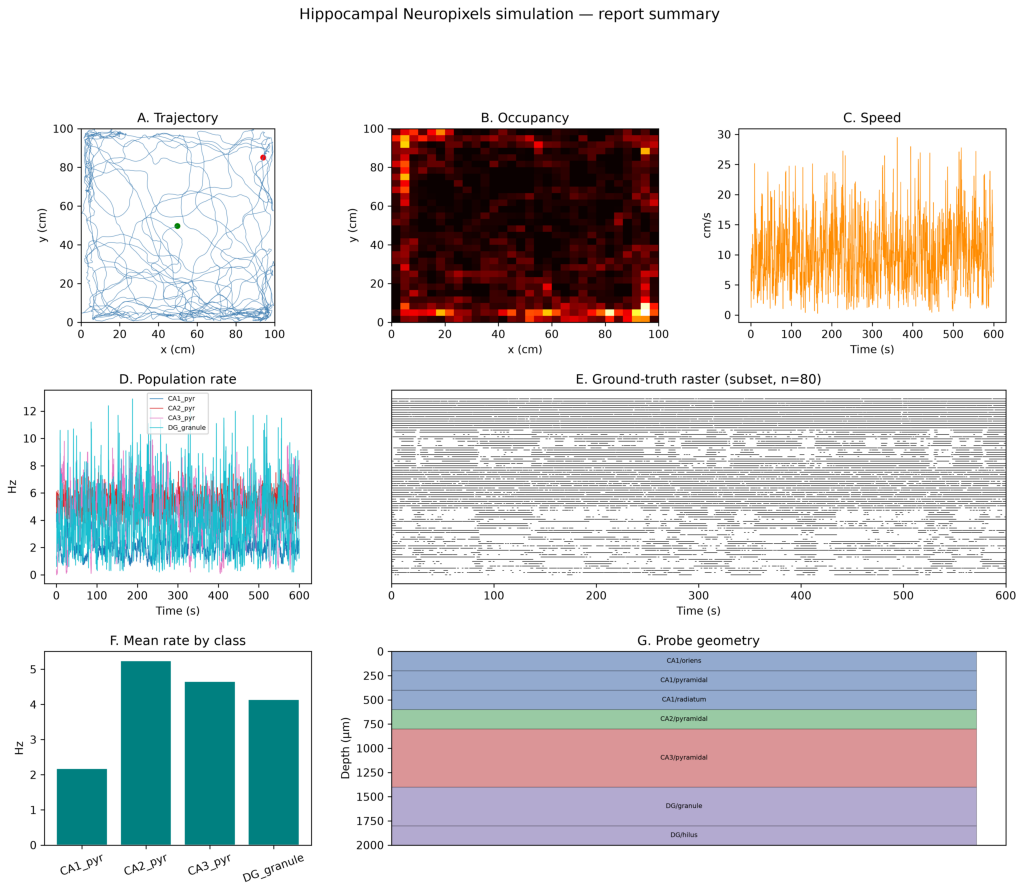
\includegraphics[width=\textwidth]{simulation_summary.png}
\caption{Composite summary of the latest hippocampal Neuropixels simulation, including trajectory, occupancy, speed, population rates, a ground-truth raster subset, mean firing rate by cell class, and probe geometry.}
\label{fig:simulation-summary}
\end{figure}

\begin{figure}[H]
\centering
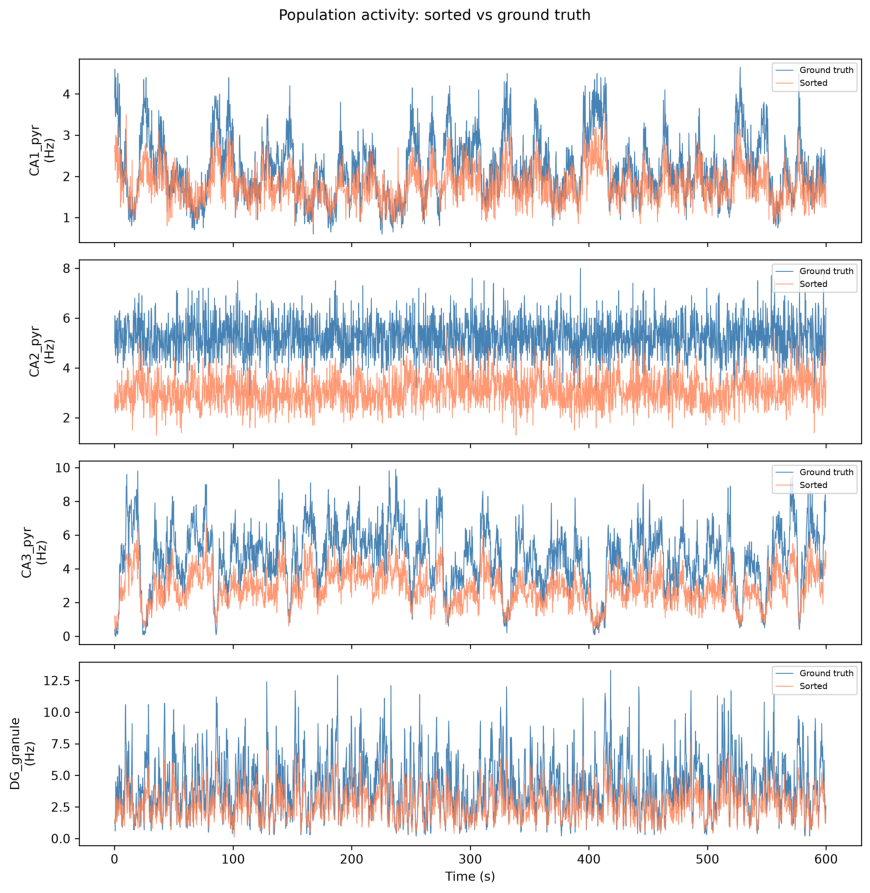
\includegraphics[width=0.82\textwidth]{sorted_vs_ground_truth_activity.png}
\caption{Population activity reconstructed from sorted spikes compared with the ground-truth population activity for each hippocampal cell class.}
\label{fig:sorted-vs-gt-activity}
\end{figure}

\begin{figure}[H]
\centering
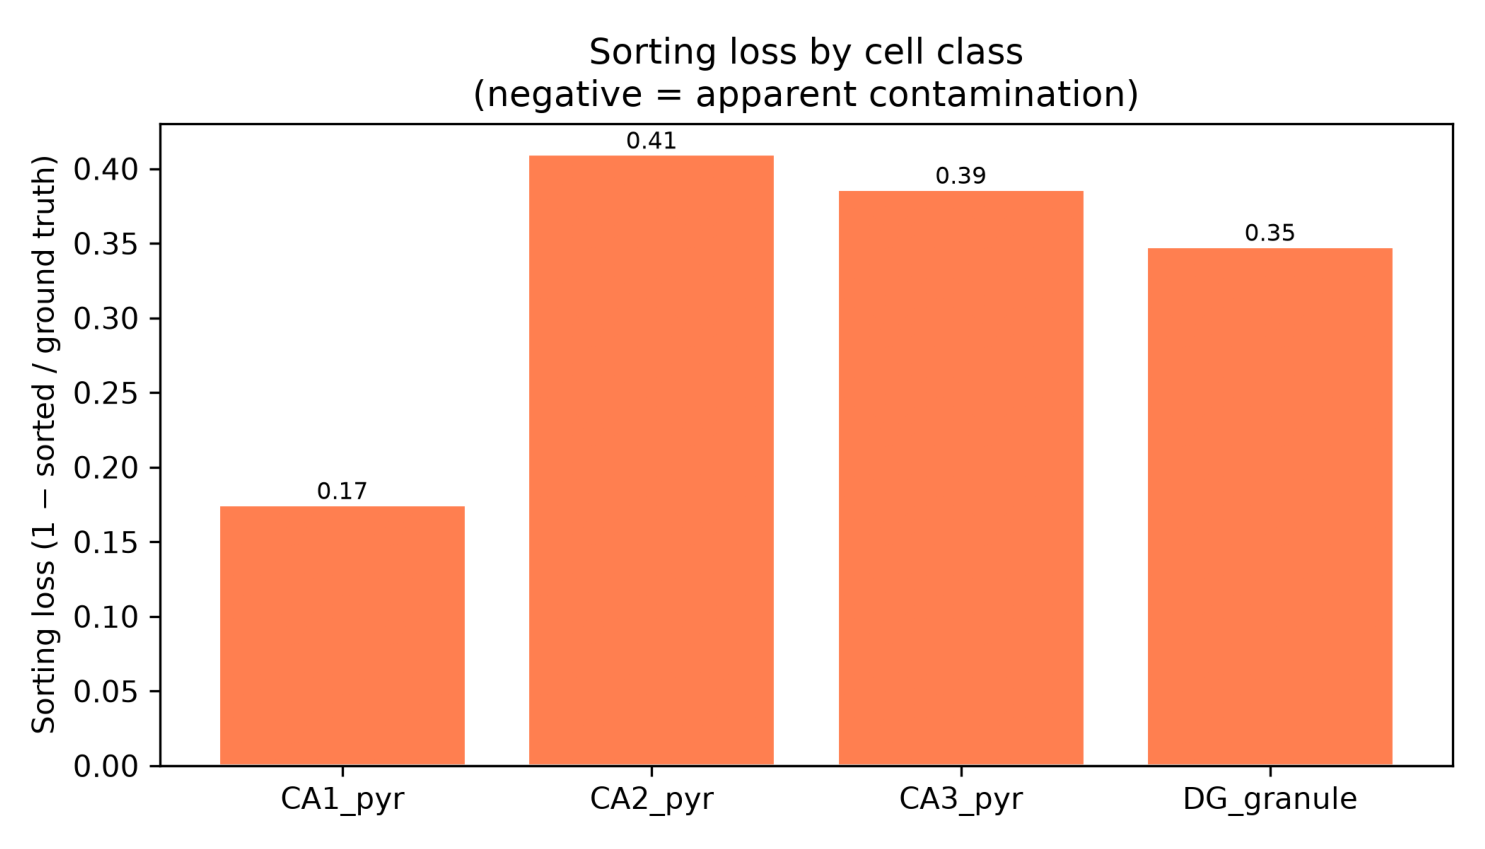
\includegraphics[width=0.82\textwidth]{sorting_loss.png}
\caption{Relative spike-count loss after Neuropixels-like recording degradation and Kilosort-like re-extraction. The latest run shows the smallest loss for CA1 pyramidal units and larger losses for CA2, CA3, and DG populations.}
\label{fig:sorting-loss}
\end{figure}

\subsection{Manifold-informed decoding}

\begin{figure}[H]
\centering
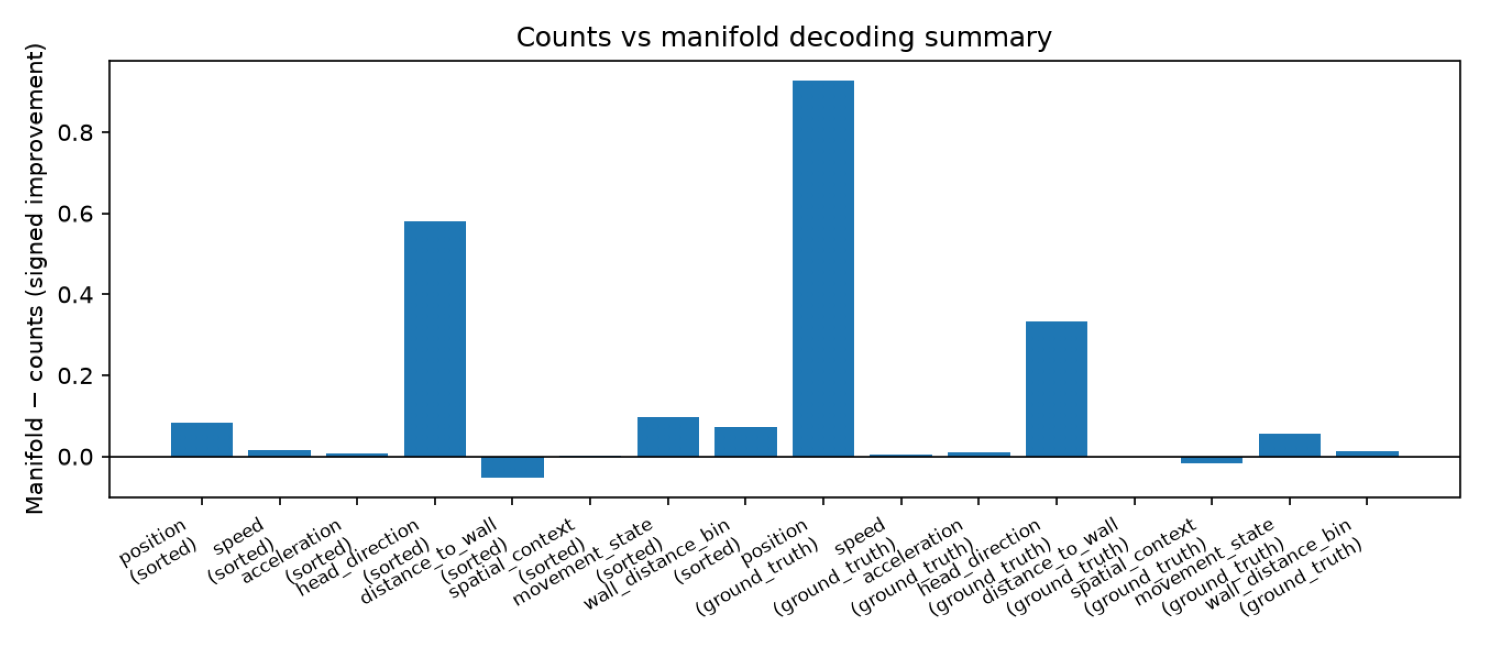
\includegraphics[width=\textwidth]{counts_vs_manifold.png}
\caption{Signed performance change for manifold features relative to raw spike counts across behavioral targets and spike sources. Positive values indicate improvement from manifold representation.}
\label{fig:counts-vs-manifold}
\end{figure}

\begin{figure}[H]
\centering
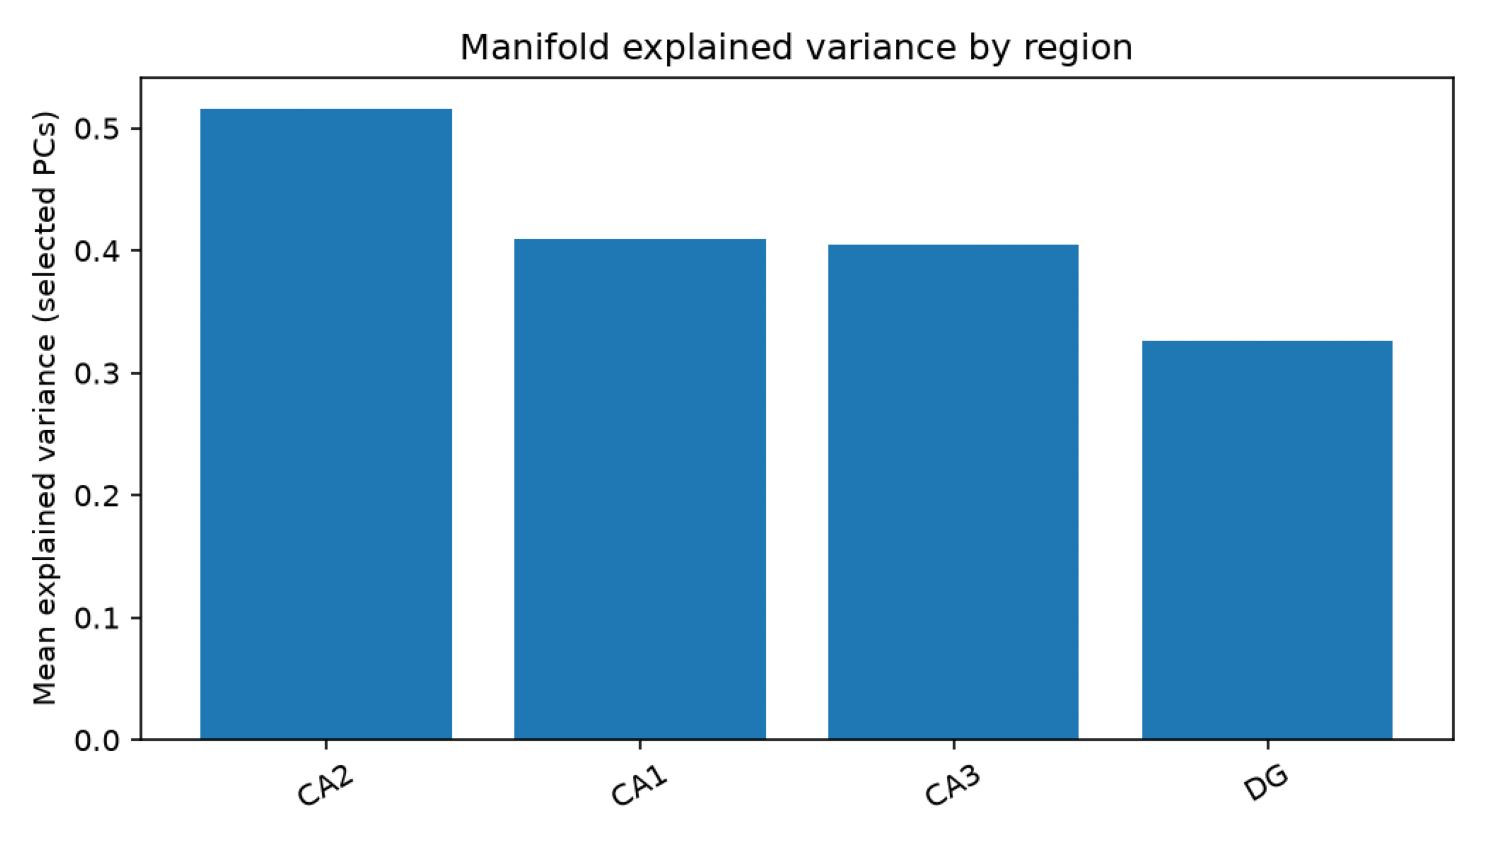
\includegraphics[width=0.82\textwidth]{manifold_variance.png}
\caption{Mean variance explained by the selected region-level PCA components. CA2 has the most compact low-dimensional representation in this run, while DG requires a larger fraction of dimensions to capture comparable variance.}
\label{fig:manifold-variance}
\end{figure}

\begin{figure}[H]
\centering
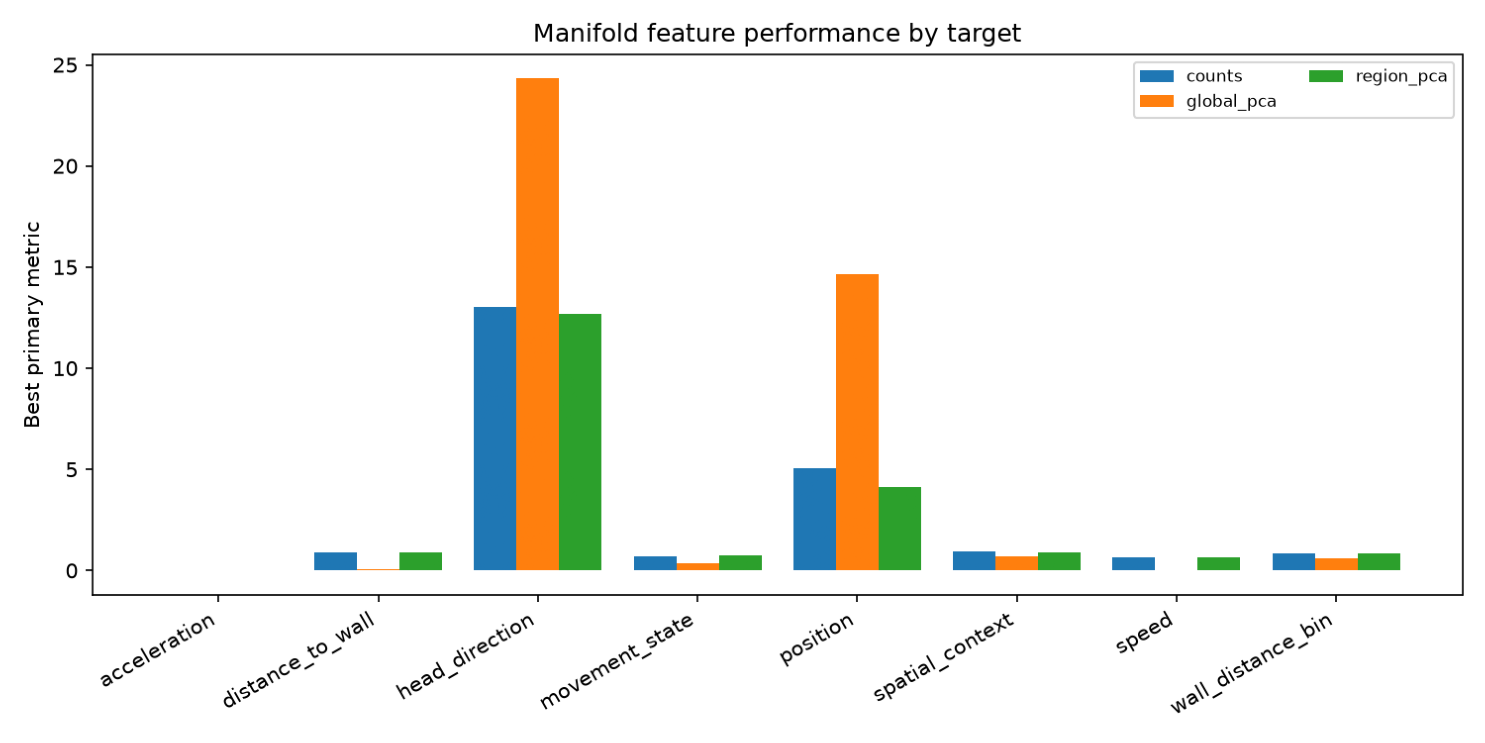
\includegraphics[width=\textwidth]{manifold_performance.png}
\caption{Best decoding metric by target for raw counts, global PCA, and region-wise PCA features. Metric direction differs by target, so this panel should be interpreted together with the target definitions in Table~\ref{tab:targets}.}
\label{fig:manifold-performance}
\end{figure}

\begin{figure}[H]
\centering
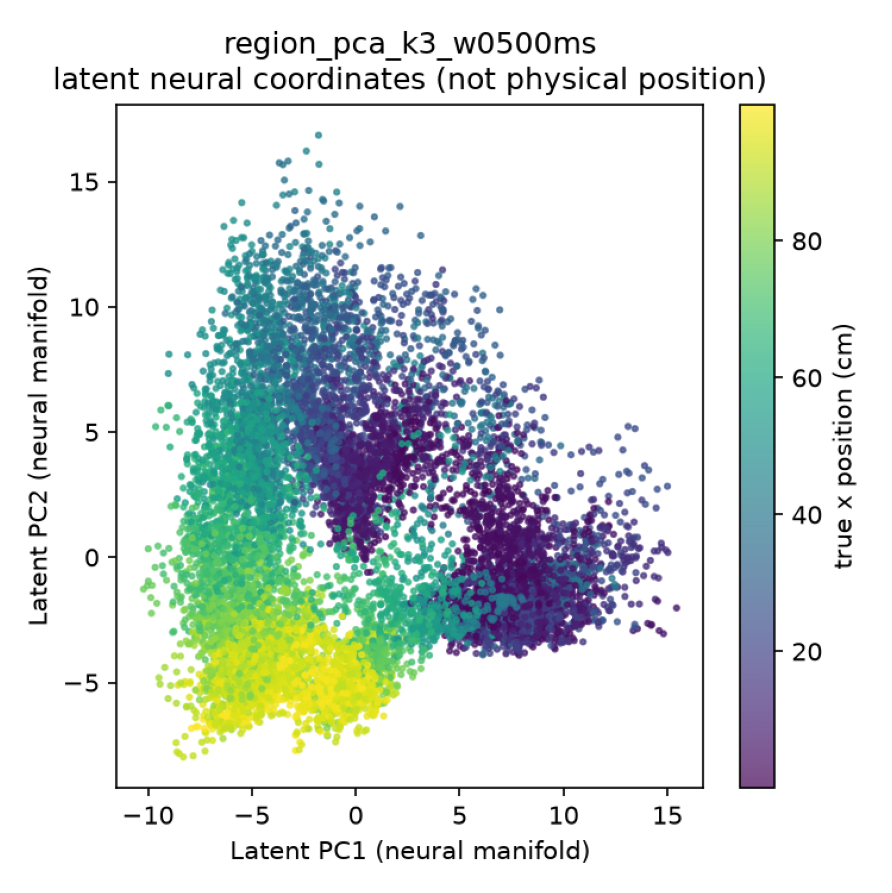
\includegraphics[width=0.70\textwidth]{region_pca_trajectory.png}
\caption{Population trajectory in the first two region-PCA coordinates, colored by true horizontal position. The structured color gradient indicates that the region-restricted latent space preserves spatial information.}
\label{fig:region-pca-trajectory}
\end{figure}

\subsection{Offline decoder selection and recording degradation}

\begin{figure}[H]
\centering
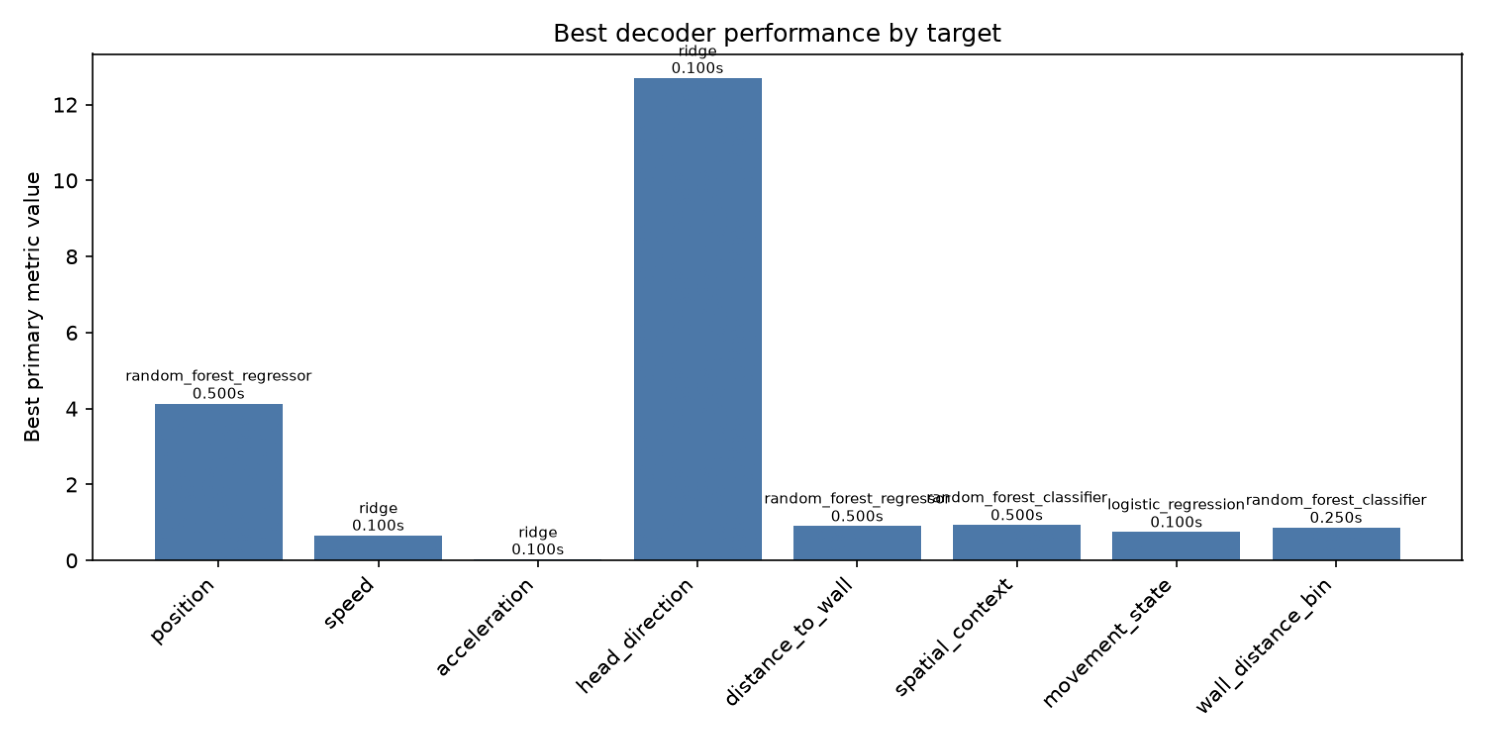
\includegraphics[width=\textwidth]{best_decoder_ground_truth.png}
\caption{Best offline decoder and integration window selected for each behavioral target using ground-truth spikes.}
\label{fig:best-decoder-gt}
\end{figure}

\begin{figure}[H]
\centering
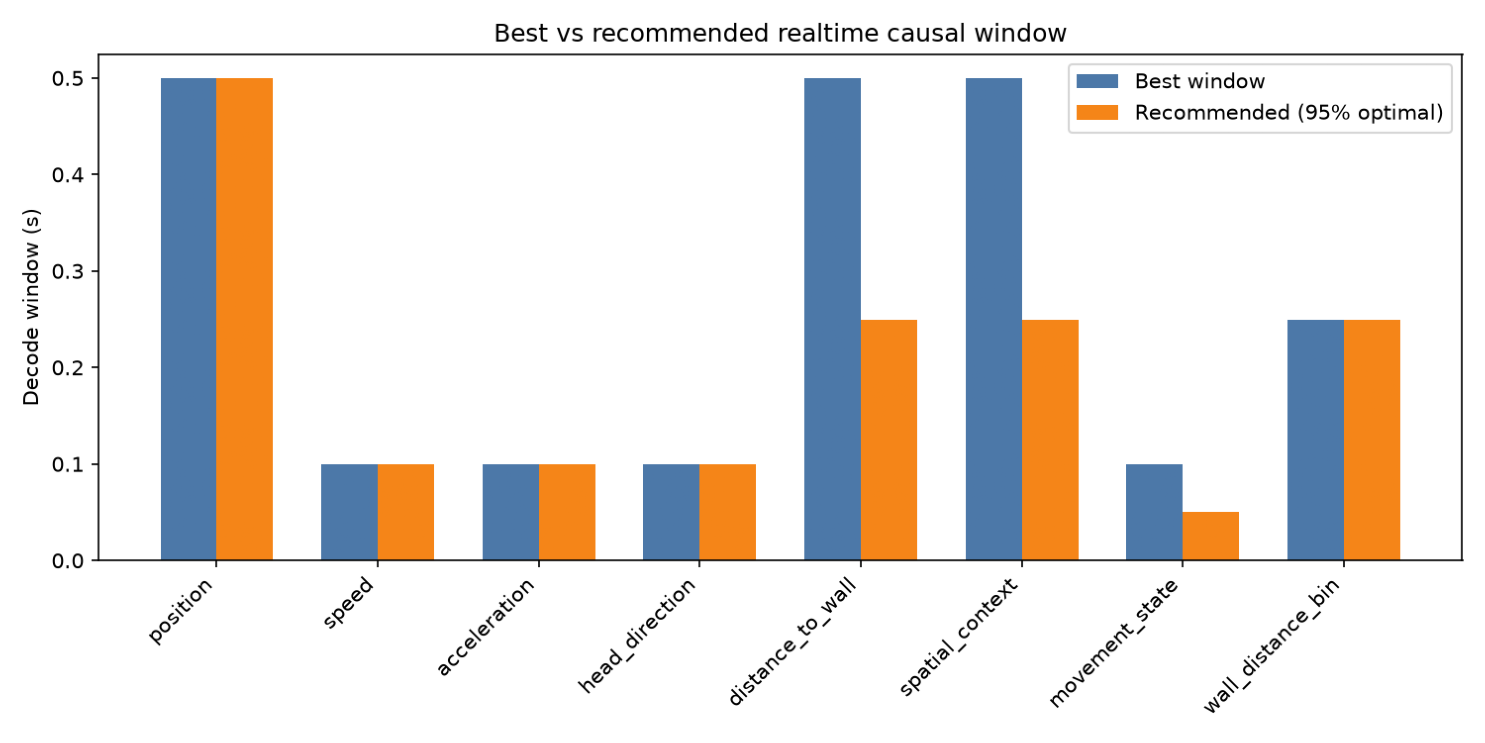
\includegraphics[width=\textwidth]{recommended_windows_ground_truth.png}
\caption{Best and shortest-near-optimal causal windows for each target. The selection policy can substantially reduce latency for distance-to-wall, spatial-context, and movement-state decoding.}
\label{fig:recommended-windows}
\end{figure}

\begin{figure}[H]
\centering
\begin{subfigure}{0.49\textwidth}
  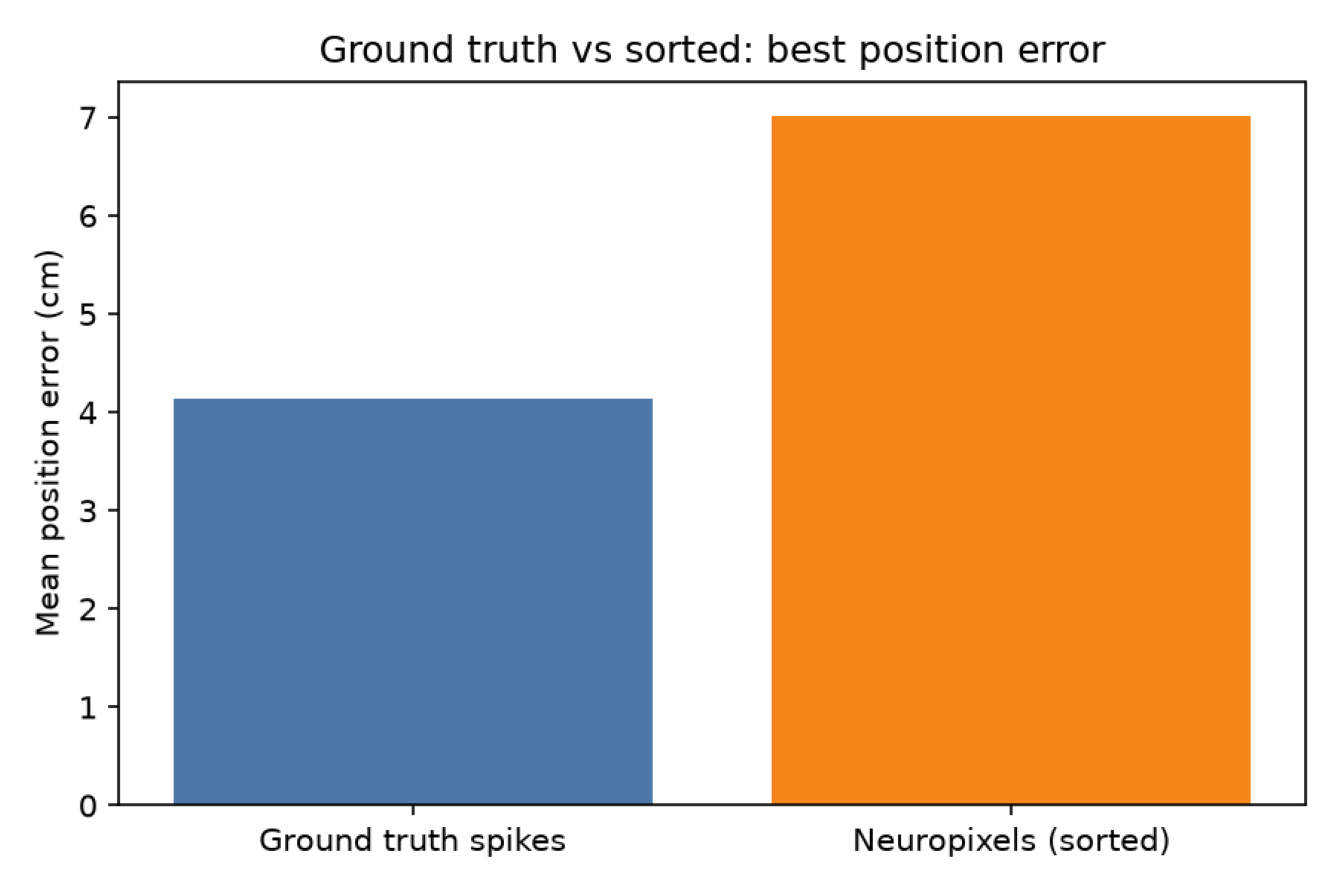
\includegraphics[width=\textwidth]{gt_vs_sorted_position.png}
  \caption{Mean position error.}
\end{subfigure}\hfill
\begin{subfigure}{0.49\textwidth}
  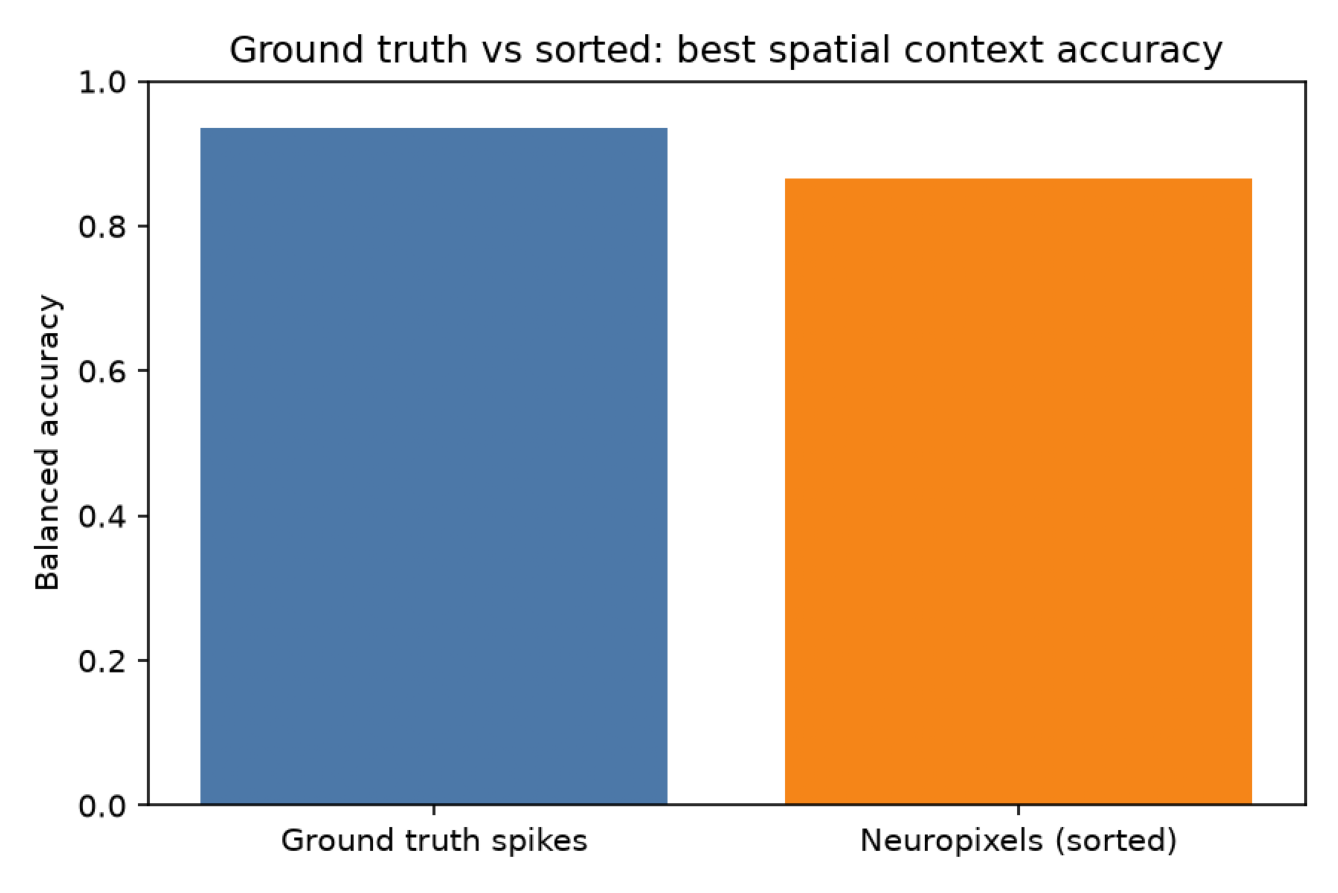
\includegraphics[width=\textwidth]{gt_vs_sorted_context.png}
  \caption{Spatial-context balanced accuracy.}
\end{subfigure}
\caption{Effect of Neuropixels-like degradation and sorting on the best offline position and spatial-context decoders.}
\label{fig:gt-vs-sorted-decoding}
\end{figure}

\subsection{Causal realtime replay}

\begin{figure}[H]
\centering
\begin{subfigure}{0.49\textwidth}
  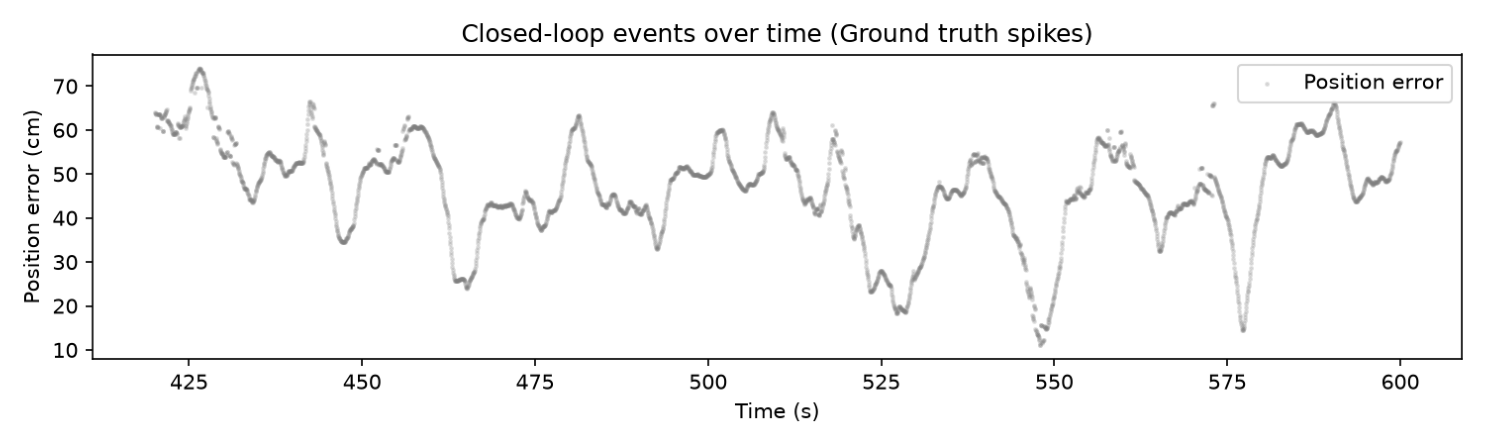
\includegraphics[width=\textwidth]{realtime_gt_events.png}
  \caption{Ground-truth spike source.}
\end{subfigure}\hfill
\begin{subfigure}{0.49\textwidth}
  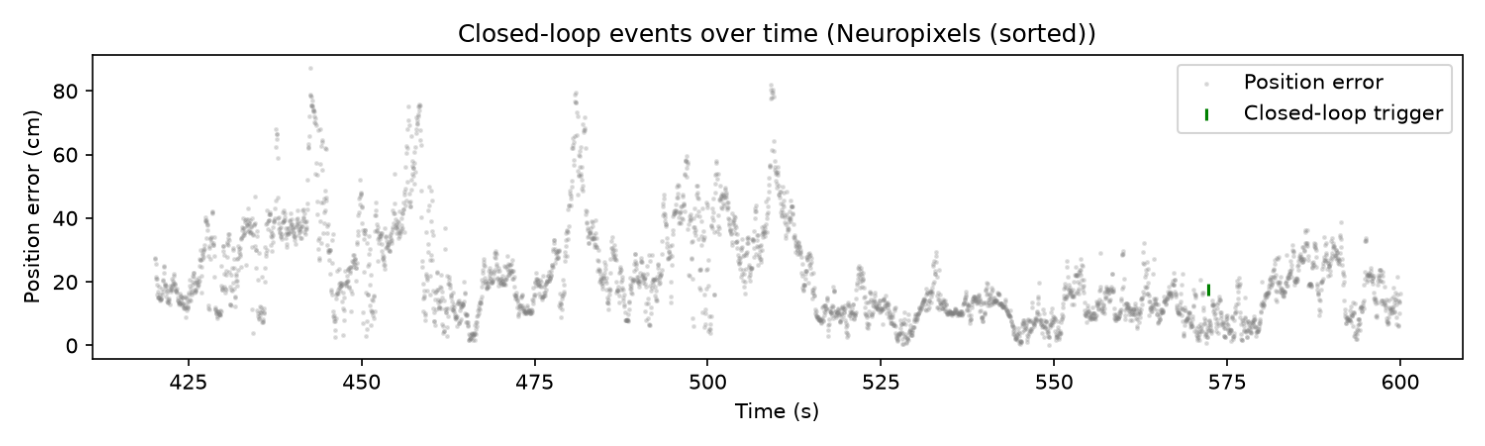
\includegraphics[width=\textwidth]{realtime_sorted_events.png}
  \caption{Sorted spike source.}
\end{subfigure}
\caption{Closed-loop events overlaid on causal realtime position error. Green and red markers indicate correct and incorrect triggers under the configured policy.}
\label{fig:closed-loop-events}
\end{figure}

\begin{figure}[H]
\centering
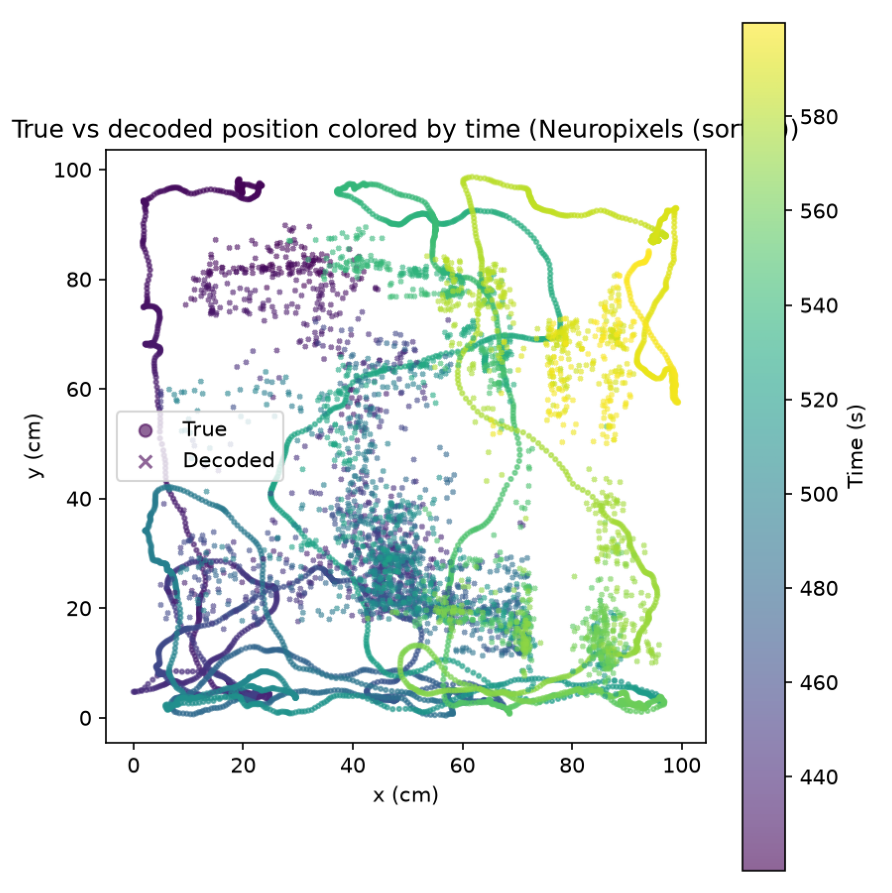
\includegraphics[width=0.72\textwidth]{realtime_sorted_position.png}
\caption{True and causally decoded position during realtime replay using Neuropixels-like sorted spikes, with both trajectories colored by time.}
\label{fig:realtime-sorted-position}
\end{figure}

% ============================================================
\section{Outputs and visualization}
% ============================================================

\begin{lstlisting}[caption={Experiment directory layout.}]
outputs/<run>/
  behavior.csv, units.csv, spikes_*.csv, summary.json
  decoder_comparison/{sorted,ground_truth}/
  realtime_decoding/{spike_source}/{target}_{policy}/
  decoding/                 # optional temporal W x L
  figures/
    decoder_comparison/
    realtime_decoding/
    output.pdf
\end{lstlisting}

\texttt{run\_visualizations.py} detects available folders and plots simulation, comparison, and realtime figures without recomputing models.
With \texttt{--compile-pdf}, all PNGs are assembled into a sectioned \texttt{figures/output.pdf}.

% ============================================================
\section{Limitations}
% ============================================================

\begin{itemize}[leftmargin=*]
  \item Simulated region functions and rate parameters are configurable hypotheses, not recovered biology.
  \item Sorted spikes lose some ground-truth metadata (identity, projections).
  \item Supervised embeddings (when added) reflect supplied labels and should not be treated as complete intrinsic geometry.
  \item Realtime-compatible methods must not use future spikes or future smoothing.
  \item Simulation results require later experimental validation.
\end{itemize}

% ============================================================
\section{Repository map (selected)}
% ============================================================

\begin{table}[h]
\centering
\caption{Selected modules.}
\label{tab:modules}
\small
\begin{tabular}{@{}ll@{}}
\toprule
Path & Role \\
\midrule
\texttt{hippo\_sim/} & Behavior, rates, spikes, recording, sorting \\
\texttt{realtime/timing.py} & $\mathrm{d}t_{\mathrm{update}}$, $W$, $L$, $\tau$ \\
\texttt{realtime/spike\_features.py} & Causal count matrices \\
\texttt{realtime/decoder\_models.py} & Model zoo \\
\texttt{realtime/bayesian\_decoder.py} & Bayesian place decoder \\
\texttt{realtime/manifold\_features.py} & Static manifold modes \\
\texttt{realtime/manifolds/} & Temporal raw / PCA encoders \\
\texttt{realtime/temporal/} & History models and W$\times$L search \\
\texttt{realtime/workflow.py} & Public decoder orchestration \\
\texttt{visualization/} & Figures and PDF compilation \\
\bottomrule
\end{tabular}
\end{table}

\vspace{1em}
\noindent\textit{License:} research / educational use.\\
\noindent\textit{Companion README:} project root \texttt{README.md} (Unicode equations for Markdown preview).

\end{document}
